\section{简介}

网络用户逐渐流失,最终瓦解了~\cite{friendster,DBLP:conf/cosn/GarciaMS13}。

\begin{figure}
    \centering
    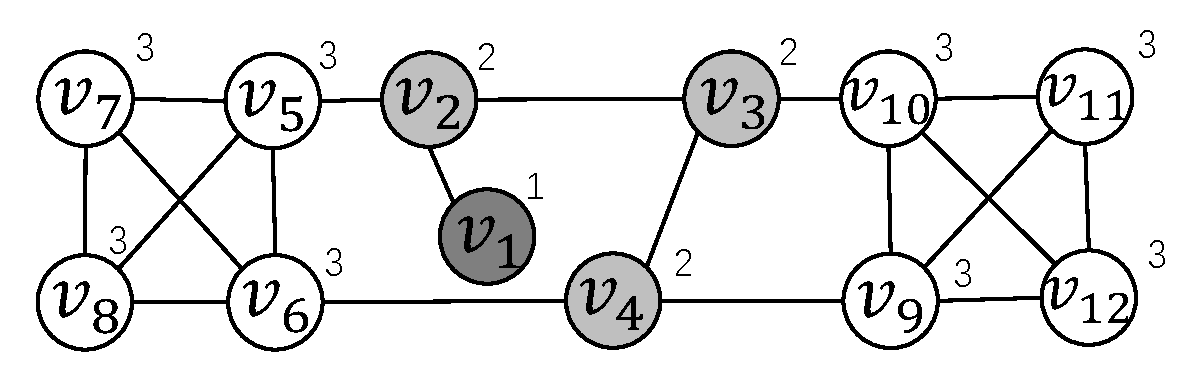
\includegraphics[width=0.7\linewidth]{figures/toy-example}
    %\vspace{-2mm}
    \caption{A Toy Graph (The coreness of each vertex is marked near the vertex)}%
    \label{fig:example}
\end{figure}

\begin{table}[t]
    \centering%
    \caption{Collapsed $k$-Core v.s. Collapsed Coreness in Figure~\ref{fig:example}}
    \label{tab:example}
    %\renewcommand{\arraystretch}{1.3}%
    %\resizebox{0.48\textwidth}{!}{
    \begin{tabular}{|l|c|c|c|c|}
        \hline
        \textbf{Problem}                    & \textbf{Input}             & \textbf{Collapser}         & \textbf{Followers}      & \textbf{Coreness}   \\
        \hline
        \hline
        \multirow{2}{*}{Collapsed $k$-Core} & $k=2,b=1$              & $v_3$                  & $v_2$               & from $2$ to $1$ \\

        \cline{2-5}                         & $k=3,b=1$              & $v_6$                  & $v_{5},v_{7},v_{8}$ & from $3$ to $2$ \\
        \hline
        \multirow{2}{*}{Collapsed Coreness} & \multirow{2}{*}{$b=1$} & \multirow{2}{*}{$v_5$} & $v_2$ & from $2$ to $1$ \\
        \cline{4-5}                         &                        &                        & $v_6,v_7,v_8$       & from $3$ to $2$ \\

        \hline
    \end{tabular}
    %}
\end{table}
